% !TeX root = scaffold-70.tex
\renewcommand{\imagepath}{../70-supervised/img}

\chapter{Supervised Analysis: Zero-Shot Classification}\label{ch:supervised}
In this chapter, the newspaper articles \todo{continue}

\section{Analysis Procedure}
In contrast to topic modelling, in the case of zero-shot classification (see section~\ref{ch:zero_shot}) training and optimization has already been performed by the model provider. The employed BART model~\autocite{lewis_bart_2020} \todo{decide for one kind of reference} is not trained on any inputs and is not altered during the classification process. It can assign a relative semantic proximity $p_{i, l}$ to a given newspaper article $i$ for each label $l$ out of a set of labels. This quasi-probability represents how close the meaning of the label is to the meaning of the article. Similar to the procedure in topic modelling, a label was assigned to an article if it had the highest proximity:
\begin{align}
    l_{i} = \max_{l'} p_{i, l'}
\end{align}
Also like in the topic modelling procedure, the information-theoretical entropy \autocite{gray_entropy_2013} for each article was calculated as a measure of how secure the model was of its prediction:
\begin{align}
    H_i = -\sum_{l'} p_{i, l'} \ln p_{i, l'}.
\end{align}
Low entropy signifies that the model could attest a very close proximity of one of the labels, hence an unambiguous assignment of label, whereas a high value of $H_i$ testifies an ambiguous association between the article and the label. As the range of $H$ depends on the number $n_\text{labels}$ of labels, the following normalized variant is used for comparing the model's security across categories:
\begin{align}
    \widetilde{H}_i = \frac{H_i}{\ln n_\text{labels}}
\end{align}

Note that in contrast to the previous chapter's concept of hypertopics, which were human assigned to word lists carrying the articles' semantic information, here the model quantifies the semantic relationship between each article and a given label.

In order to examine the article texts with respect to the aspects motivated in section~\ref{ch:this_thesis}, namely topic, sentiment, success, delinquency, and journalistic style, for each of these aspects one or more categories and a corresponding set of labels was compiled based on the author's intuition and on what would seem interesting for the analysis of role model qualities. The labels used in the analysis are presented in section~\ref{ch:supervised_results} for each category.

\begin{figure}
    \centering
    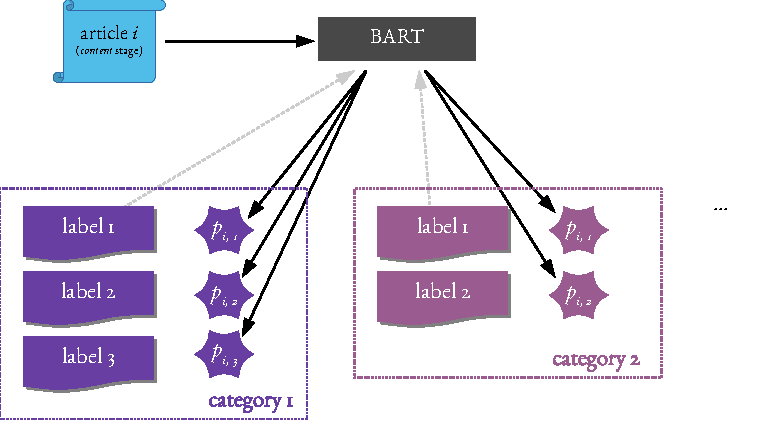
\includegraphics[]{\imagepath/zero_shot_schema.pdf}
    \caption{Schematic of the zero shot classification procedure: An article $i$ is fed into the BART model along with a set of labels, called a category. BART then assigns a relative proximity $p$ to each label for this article. This is repeated for different categories, each having a different set of labels. The BART model itself doesn't depend on any input and is not altered during the whole process.}\label{fig:zero_shot_schema}
\end{figure}

The classification procedure is illustrated in figure~\ref{fig:zero_shot_schema}. The BART model was integrated as suggested in \textcite{huggingfacebart-large-mnli_facebookbart-large-mnli_nodate}. As an input to the model the text in the \textit{content} stage was used, i.e. with most structure of the human language preserved.

\section{Accuracy}\label{ch:supervised_accuracy}
In a first evaluation step, the accuracy of the zero-shot classification was assessed using the human annotated data. To this end, the model made a prediction for each article from the set of labels used in the human annotation process, namely \textit{life}, \textit{movie}, \textit{music}, and \textit{sports}. An accuracy (cf. equation~\eqref{eq:accuracy}) of \SI{57.9}{\percent} was achieved, human annotation and the model-predicted labels are compared in the confusion matrix in figure~\ref{fig:zero_shot_confusion_matrix_topic}, showing that the model especially counts articles that the human annotator marked as sport-related to the label \textit{life}. It was conjectured that this might stem from an alledged semantic proximity of the word ``life'' with ``live sports''. Therefore an alternative set of labels with the \textit{life} label exchanged for \textit{social} was checked. For it an almost equal accuracy of \SI{55.9}{\percent} was achieved, the confusion matrix is shown in figure~\ref{fig:zero_shot_confusion_matrix_topic_l}. Indeed this reduced the confusion with the \textit{label}, however now there was a more pronounced confusion of \textit{social} and \textit{movie}, which is also not surprising considering that reports about movie plots often convey social aspects. Looking at the averaged normalized entropies showed that the model makes more convinced predictions if \textit{life} is replaced by \textit{social}, $\Braket{\widetilde{H}}_\text{life} = 0.87 > 0.77 = \Braket{\widetilde{H}}_\text{social}$.

\begin{figure}
    \centering
    \begin{subfigure}{0.48\textwidth}
        \centering
        \includegraphics[]{\imagepath/zero_shot_confusion_matrix_topic.pdf}
        \caption{topic}\label{fig:zero_shot_confusion_matrix_topic}
    \end{subfigure}
    \hspace{0.03\textwidth}
    \begin{subfigure}{0.48\textwidth}
        \centering
        \includegraphics[]{\imagepath/zero_shot_confusion_matrix_topic_l.pdf}
        \caption{topic (soc.)}\label{fig:zero_shot_confusion_matrix_topic_l}
    \end{subfigure}
    \caption{Comparison of the model prediction and the human annotation for the topic and topic (soc.) categories. An accuracy of \SI{}{\percent} was achieved in predicting the human annotation labels. The most pronounced mistake is that the model classifies ...}\label{fig:zero_shot_confusion_matrices}
\end{figure}

The accuracy of the zero-shot approach is hence less than in the topic modelling approach with a pre-trained model (\SI{76}{\percent}). However, the qualitative accuracy recognizable from the confusion matrices is remarkable given that the has not been trained on the corpus of newspaper articles. Since the articles' topics are not unambiguous and also the human-annotated labels are thus subject to uncertainty, the zero-shot approach is arguably still very promising despite its lower accuracy, especially given that it makes it possible to explore all the non-topic aspects of newspaper articles scrutinized in the following.


\section{Results}\label{ch:supervised_results}
In total, the model assigned labels from twelve categories to each article. As was done in the evaluation of topic modelling, the distribution of the articles across the labels of each category was then compared for the low-\gls{ses} and the high-\gls{ses} groups.

Again, a $\chi^2$ contingency test was used to identify significant differences between the article distributions (cf. equation~\eqref{eq:h0_contingency}):
\begin{align}
    \begin{split}
        H_{0, \text{contingency}}: ~~~ &\text{distributions } p_{s, l} \text{ over labels } l \text{ are indepedent of } s\\
    & \text{i.e. } p_{s, l} = p_s \cdot p_l ~~ \forall l, s
    \end{split}
\end{align}
A set of per-label $\chi^2$ tests were conducted to find significant differences in the amount of articles per label were looked for (cf. equation~\eqref{eq:h0_topic}):
\begin{align}
    \begin{split}
        H_{0, \text{ label }l}: ~~~ &\text{number of articles } n_{s, l} \text{ equals expected number } \tilde n_{s, l} \\
        & \text{i.e. } n_{\text{low}, l} = \tilde n_{\text{low}, l} \text{ and } n_{\text{high}, l} = \tilde n_{\text{high}, l},
    \end{split}
\end{align}
with the number of articles $n_s$ in \gls{ses} group $s$, the number of articles $n_l$ associated with label $l$, the total number $n$ of articles, and the expected number of articles $\tilde n_{s, l} = n_s \cdot \frac{n_l}{n}$ per label $l$ and \gls{ses} $s$ assuming independence from \gls{ses}.

\begin{table}
    \centering
    \resizebox{0.85\textwidth}{!}{../../../build/thesis/70-supervised/zero_shot_result_table.tex}
    \caption{Results of the zero-shot classification for each category along with $\chi^2$ contingency and per-label tests. Legend: $\Braket{\widetilde{H}}$ is the average of the normalized entropy $\widetilde{H}$.}\label{tab:zero_shot_result_table}
\end{table}

\paragraph{Topics}
\paragraph{Sentiment}
\paragraph{Success}
\paragraph{Relatability}
\paragraph{Delinquency}
\paragraph{Newspaper Coverage}

\section{Discussion}